% FairMind-E position paper for GREENS 2027 (ICSE 2027 workshop): camera-ready
% draft. paper.tex is the version submitted as HotCRP #43 on 2026-11-11 and is
% kept unchanged as the record of what reviewers read.
%
% Changes from paper.tex:
%  - references replaced with the verified list from ../ccai2026/submission.tex
%  - policy text matches the engine on main (class-midpoint confidence; a
%    tracker in load-model fallback is classed manual)
%  - new subsection on the gate misclassifying its own degraded tracker
%  - method disagreement reported with a statistic that does not depend on
%    the FLOP model's placeholder constant (analysis/hypotheses.py,
%    factor_after_best_rescale)
%  - Fig. 2 caption matches the figure (physical reruns only)
%  - four authors, as on HotCRP; unit-test count updated to 59
% Figures come from ../ccai2026/figures (analysis/make_figures.py).

\documentclass[10pt,conference]{IEEEtran}

\usepackage[utf8]{inputenc}
\usepackage[T1]{fontenc}
\usepackage{cite}
\usepackage{amsmath}
\usepackage{graphicx}
\usepackage{booktabs}
\usepackage{url}
\usepackage[hidelinks]{hyperref}
\graphicspath{{../ccai2026/figures/}}

\newcommand{\sysname}{FairMind-E}

\begin{document}

\title{Release Gates Should Ask\\Where the Carbon Number Came From}

\author{\IEEEauthorblockN{Adhithya Rajasekaran, Dhinakaran Thangaraj, Lakshman S, Navya Velicheti}
\IEEEauthorblockA{Axonome\\
Corresponding author: adhi.r@axonome.xyz (ORCID 0009-0004-1682-7958)}}

\maketitle

\begin{abstract}
Green software practice increasingly puts a carbon number in front of a release
decision: a carbon budget, a readiness level, or a risk rating. None of these
gates asks whether the number itself can be trusted. We argue that the
\emph{provenance} of an environmental claim should be a first-class release
criterion, and we report on \sysname, an environmental release gate shipped
inside FairMind, an open-source AI governance platform. A confidence score
fixed by provenance class, crossed with an impact tier, resolves to \emph{go},
\emph{conditional\_go}, or \emph{no\_go} and blocks the platform's
deployment-approval workflow. In a measurement study over four workloads, a
software power tracker and an analytic FLOP model disagreed in direction from
one workload to the next; no choice of the FLOP model's free constant brings
them within a factor of 4.7 on every workload. The study also caught our own
gate passing a weak number: the tracker had fallen back to a CPU-load model,
yet the gate, which keyed provenance on tool identity, gave it high confidence
and an unconditional \emph{go} on all 20 runs. Finally, casting a fine-tune to
\texttt{bfloat16} on a host with no optimised kernel made it 46 times slower,
so a gate that accepts declared mitigations would have logged a reduction that
never happened. Both failures argue for deriving provenance from how a number
was produced, and for re-measuring mitigations before crediting them.
\end{abstract}

\begin{IEEEkeywords}
green software, sustainable AI, release engineering, carbon measurement,
evidence quality, AI governance
\end{IEEEkeywords}

\section{Position}

Software teams are being asked to account for the energy and carbon of the AI
systems they ship. Standards bodies are building the measurement layer:
quantification-methods inventories~\cite{cen18145}, sustainability
overviews~\cite{iso20226}, and a G7-commissioned inventory of thirteen
measurement and reporting initiatives~\cite{g7}. The EU AI Act anticipates
harmonised standards for reporting AI resource performance (Article~40) and
requires general-purpose model documentation to state known or estimated energy
consumption (Annex~XI)~\cite{aiact,ebert}. None of these instruments says how
the \emph{quality} of an environmental claim should condition a deployment
decision.

Proposed carbon-aware gates decide on magnitude. Carbon-aware governance gates
embed carbon budgets in the governance layer and record energy provenance in
audit logs, but do not let it change the decision~\cite{cagg}; region-aware
sustainability pyramids gate on readiness levels~\cite{gtrace}; risk
integrations treat AI carbon as one risk dimension~\cite{tkachenko}. Yet
measurement research shows reliability varies sharply with disclosure:
metadata-completeness tiers across 5{,}227 public models span roughly
$1.2\times$ to $2\times$ estimation error~\cite{huggingcarbon}, and spend-based
fallbacks in tiered accounting for purchased inference overestimate by
10--40$\times$~\cite{scope3}. Recent work acts on the \emph{statistical spread}
of an estimate, through calibrated cost and carbon prediction for agentic
systems~\cite{greensarc} or confidence-gated filtering of emissions
predictions~\cite{trustpems}. None acts on \emph{where the number came from}, so
a precise-looking figure from a weak source passes every published gate while
sitting comfortably under budget.

Our position is narrow: \textbf{for green software engineering, evidence
quality, not only impact magnitude, should gate a release.} The idea is old in
life-cycle assessment, where pedigree matrices grade the provenance of an
inventory figure~\cite{weidema} and the NUSAP pedigree qualifies
uncertainty~\cite{nusap}; recent work recommends indicator-style disclosure for
AI-assisted footprinting but proposes no score, threshold, or
gate~\cite{credible}. We bring it into the release pipeline, where software
engineers already make go or no-go decisions.

\section{Mechanism}

\paragraph{Provenance classes and confidence} Every assessment declares its
measurement source, normalised to one of five provenance classes with bounded
confidence: \emph{measured} (hardware telemetry; 0.85--1.00),
\emph{tool\_estimated} (software power trackers reading hardware counters;
0.60--0.85), \emph{vendor\_reported} (cloud-provider figures; 0.40--0.60),
\emph{manual} (analytic estimates, including a tracker that has fallen back to
a load-times-TDP model; 0.20--0.40), and \emph{unknown} (0.0). Confidence is
fixed at the class midpoint: a caller-supplied score is recorded for audit but
never enters the gate. Provenance is reported separately from quantified
uncertainty, so a narrow interval cannot launder a weak source.

\paragraph{Tiers and the decision matrix} Metrics map to low, medium, or high
impact per lifecycle phase, using location-based carbon so market instruments
cannot lower a gate outcome. Confidence bands (\emph{high} $\geq 0.70$;
\emph{moderate} $0.35 \leq c < 0.70$; \emph{low} $0 < c < 0.35$;
\emph{undisclosed} $c = 0$)\footnote{The engine names these bands
\texttt{measured}, \texttt{estimated}, and \texttt{unknown}; we rename them
here so they do not collide with the provenance classes.} cross with impact
tiers into the matrix in Fig.~\ref{fig:main}(b). Confidence 0.0 short-circuits
to \emph{no\_go}: an undisclosed claim never passes. The matrix is deliberately
asymmetric: \emph{vendor\_reported} evidence tops out in \emph{moderate}, so a
medium-impact workload assessed only from provider figures never receives an
unconditional \emph{go}, and no evidence earns a high-impact release more than
\emph{conditional\_go}. A \emph{conditional\_go} cannot be approved until it
carries a dated, owned mitigation or an explicit exception with owner, expiry,
and rationale, so reviewer overrides are auditable rather than informal. Six
controls (ENV-1 to ENV-6: boundary, energy accounting, dual location and market
carbon, per-functional-unit efficiency, evidence confidence with disclosed
uncertainty, and mitigation or exception) define coverage. Disclosed offsets
are recorded but never subtracted and never improve a gate outcome.

\section{Implementation in a release pipeline}

\sysname{} ships inside FairMind rather than as a standalone proposal. The
decision engine is a framework-agnostic Python package with 59 unit tests
covering every matrix cell, band boundary, provenance class, and the
undisclosed-evidence short-circuit. Assessments persist as versioned governance
evidence. A release gate hooks the platform's deployment-approval workflow and
returns HTTP 409 with the blocking reason when the latest assessment is
\emph{no\_go} or an unmitigated \emph{conditional\_go}, the same way a failing
test blocks a merge. Reviewers see the matrix position, control coverage,
mitigations, and version trail; disclosures export in a shape aligned with the
European climate reporting standard~\cite{csrd}.

A 14-case hand-labelled fixture set spanning all matrix cells, mitigation
states, exception paths, and offset disclosures serves as a conformance test:
the implementation reproduces 14/14 labels. Because the same authors wrote the
fixtures, labels, and engine, this shows only that the code implements the
stated policy, not that the policy decides correctly.

\section{Measurement study}

\begin{figure}[t]
  \centering
  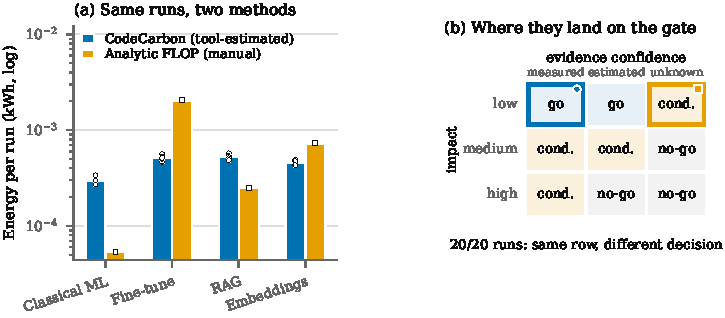
\includegraphics[width=\linewidth]{fig1_provenance_decides.pdf}
  \caption{Four workloads, five iterations each, every run assessed twice.
  (a) Energy per run by method; points are iterations, bars their means. The
  ratio between methods runs from $0.18\times$ to $3.97\times$ by workload.
  (b) Where the runs landed under the policy in force when they were gated,
  which keyed provenance on tool identity: the degraded tracker was classed
  \emph{tool\_estimated} and passed unconditionally (Section~IV).
  Under the corrected policy both methods land in the \emph{low} column.}
  \label{fig:main}
\end{figure}

Four workloads (classical ML training, transformer fine-tune, RAG inference,
batch embeddings) ran five iterations each on one host (Apple M1 Pro; seed
1337; warm-up discarded). Every run was assessed by the codecarbon software
power tracker and a documented analytic FLOP model; cloud billing was also
requested but lags execution, so its 20 records are explicit ``unavailable''
entries rather than invented figures. All runs were replayed through the
production engine, not a reimplementation.

\paragraph{The methods disagree, and not by a constant} The FLOP model reports
$0.18\times$ the tracker's energy on classical ML, $0.48\times$ on RAG,
$1.58\times$ on batch embeddings, and $3.97\times$ on the fine-tune
(geometric means over iterations). The FLOP model contains a placeholder
efficiency constant (4.0~GFLOP/s per watt), so its absolute level, and any MAPE
computed from it (123--169 percent here, depending on reference), is partly an
artifact of that choice. The \emph{spread} is not: rescaling either method by
the best possible constant still leaves them a factor of 4.7 apart at the
extremes. The reason is visible in the tracker's own output. With no hardware
counters it ran in load-model fallback, and its implied power was 23.5--27.2~W
on every workload, so it effectively measured wall-clock time. The FLOP model
counts arithmetic. The two plausibly diverge by each workload's arithmetic
intensity: classical ML spends much of its time in solver and interpreter
overhead the FLOP count ignores, while the fine-tune is arithmetic-heavy. Two methods a practitioner
might reasonably choose disagree in direction, not just in degree.

\paragraph{The gate passed its own degraded tracker} Under the
policy in force when these runs were gated (release v0.3.0-alpha), provenance
was keyed on tool identity. Codecarbon is a power tracker, so it was classed
\emph{tool\_estimated}, confidence 0.72, \emph{high} band, \emph{go}; the FLOP
model was \emph{manual}, 0.30, \emph{low} band, \emph{conditional\_go}, on all
20 runs (Fig.~\ref{fig:main}(b)). But the tracker's figure was itself a
load-times-TDP model, an analytic estimate in kind. The gate gave an
unconditional release to exactly the kind of weak source it exists to catch,
because it trusted the tool's name rather than how the number was produced. A
second defect let a caller-supplied score move within a class across the 0.35
band boundary. We closed both: the measurement harness now detects the
tracker's fallback mode and records the run as \emph{manual}, and confidence is
the class midpoint whatever score the caller claims. Under the corrected policy
both methods here land in \emph{conditional\_go}. The lesson for green software
engineering is that provenance has to be \emph{observed by the pipeline}, not
declared by the tool or the team, or the provenance check becomes one more
self-reported number.

\begin{figure}[t]
  \centering
  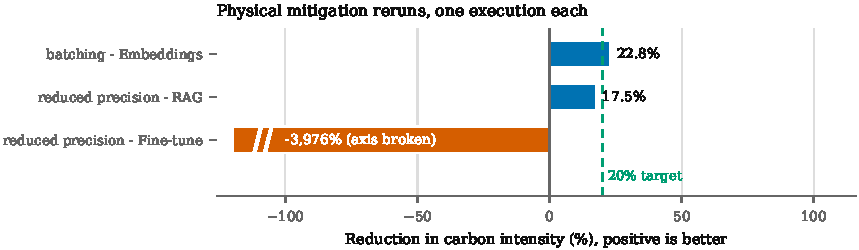
\includegraphics[width=\linewidth]{fig2_mitigations.pdf}
  \caption{The three physical mitigation reruns, one execution each ($n=1$, so
  no interval is drawn). Casting the fine-tune to \texttt{bfloat16} on a host
  with no optimised kernel took it from 62.7\,s to 2887.6\,s; its bar is
  clipped at the break mark. Region- and time-shift accounting scenarios are
  not shown: they recompute one run against placeholder emission factors and
  are not measurements.}
  \label{fig:mitigations}
\end{figure}

\paragraph{Mitigations} Only three mitigations were physical reruns
(Fig.~\ref{fig:mitigations}), each a single execution. Batching cut intensity
22.8 percent and a reduced-precision cast on RAG 17.5 percent. The third
inverted: casting the fine-tune to \texttt{bfloat16} made it 46 times slower on
a CPU with no native \texttt{bfloat16} kernel, so the cast ran in software
emulation, and the tracker estimated roughly 41 times the energy. The runtime
regression is measured directly; the energy figure largely follows from it,
since a load-based power model multiplies utilisation by time. On accelerators
with native \texttt{bfloat16} the same cast would likely have saved energy. The
point is not that the intervention is bad, but that ``we reduced precision,
therefore we cut carbon'' is routine, plausible, and here false in the harmful
direction. This is why ENV-6 requires a mitigation to be re-measured rather
than declared.

\section{Implications for green software engineering}

\paragraph{Derive provenance, do not declare it} Our own defect shows that a
provenance field filled in from a tool name is no better than a self-reported
confidence score. Pipelines should infer the class from what the measurement
actually did: which counters were read, which fallback ran.

\paragraph{Treat mitigations like code changes} A mitigation is a claim about a
change. Like a performance fix, it should be re-measured in the pipeline before
it is credited, because the effect of a precision cast or a batching change
depends on the hardware and kernels underneath.

\paragraph{Make measurement the cheapest path to release} When evidence
quality gates a release, a team that cannot substantiate its number cannot ship
unconditionally, so measuring becomes cheaper than arguing. This does not cut
emissions by itself; it makes reported reductions verifiable, and therefore
something a team can act on.

\paragraph{Open questions for the workshop} Most developer laptops and many
cloud VMs expose no energy counters, so under the corrected policy their
evidence is \emph{manual} and \emph{conditional\_go} becomes the default. Should
low-impact releases be exempt on materiality grounds, given that our benchmark
runs sit six orders of magnitude below the low-tier ceiling? Should a cloud
provider's figure (\emph{vendor\_reported}) outrank a locally run tracker in
fallback, as it does now? And how should the hierarchy be calibrated against an
independent power reference?

\paragraph{Limitations} The host exposes no accessible hardware energy
counters, so the study compares an estimate with an estimate and never claims
the \emph{measured} class. Benchmark workloads exercise only the low-impact
row, the FLOP model uses placeholder constants, the mitigation reruns are
single executions, and confidence is not yet calibrated against an independent
power reference. A first calibration attempt with \texttt{powermetrics} was
discarded because background load contaminated 19 of 20 runs; a rerun on a
quiet host, and a 15-reviewer expert panel already designed, are the next
steps. Code, run data, and analysis scripts are public in the FairMind
repository (\url{https://github.com/adhit-r/fairmind}); the study runs are
archived as release v0.3.0-alpha (doi:10.5281/zenodo.24043235), and the
corrected policy as release v0.4.1-alpha (doi:10.5281/zenodo.24274724).

\section*{Acknowledgment}
FairMind is developed at Axonome, where the authors work; the work received no
external funding. Generative AI tools (Claude, through Claude Code) assisted
with code and drafting; the authors reviewed all output and are responsible for
the content.

\begin{thebibliography}{99}
\footnotesize
\bibitem{cen18145} CEN/CLC/TR 18145:2025, \emph{Environmentally sustainable
artificial intelligence}. CEN-CENELEC, 2025.
\bibitem{iso20226} ISO/IEC TR 20226:2025, \emph{Information technology:
artificial intelligence: environmental sustainability aspects of AI systems}.
ISO/IEC, 2025.
\bibitem{g7} G7 French Presidency, \emph{Overview of initiatives for the
measurement and monitoring of energy and resource use of AI models}, May 2026.
\bibitem{aiact} Regulation (EU) 2024/1689 (Artificial Intelligence Act),
Article 40 and Annex XI \S1(2d), 2024.
\bibitem{ebert} K. Ebert, B. Gamazaychikov, P. Hacker, and S. Luccioni, ``The
global landscape of environmental AI regulation: from the cost of reasoning to
a right to green AI,'' arXiv:2603.00068, 2026.
\bibitem{cagg} M. A. Abbasi, T. J. Mikkonen, P. J. Ihantola, M. Waseem,
P. Abrahamsson, and N. K. M\"akitalo, ``Carbon-aware governance gates: an
architecture for sustainable GenAI development,'' in \emph{Proc. IEEE ICSA
Companion (ICSA-C)}, 2026, pp. 341--345, arXiv:2602.19718.
\bibitem{gtrace} Z. Kausar, S. Latif, R. K. Shahzad, and M. Fatima,
``Quantifying the climate risk of generative AI: region-aware carbon accounting
with G-TRACE and the AI sustainability pyramid,'' arXiv:2511.04776, 2025.
\bibitem{tkachenko} N. Tkachenko, ``Integrating AI's carbon footprint into risk
management frameworks: strategies and tools for sustainable compliance in
banking sector,'' arXiv:2410.01818, 2024.
\bibitem{huggingcarbon} X. Wang, R. Ming, J. Qiu, J. Zhao, and J. Gu,
``Hugging Carbon: quantifying the training carbon emissions of AI models at
scale,'' arXiv:2605.01549, 2026.
\bibitem{scope3} G. Llopis-Garcia, ``Accounting for purchased artificial
intelligence inference in corporate greenhouse gas inventories: a token-based
method,'' arXiv:2606.10660, 2026.
\bibitem{greensarc} G. Besanson, ``Green SARC: predictive cost and carbon
governance for agentic AI systems,'' arXiv:2606.15954, 2026.
\bibitem{trustpems} R. Potts, A. Durrant, R. Hackney, and G. Leontidis,
``Trust-aware predictive emissions monitoring for gas turbine fleets with
limited labelled data,'' arXiv:2606.06156, 2026.
\bibitem{weidema} B. P. Weidema and M. S. Wesn\ae s, ``Data quality management
for life cycle inventories: an example of using data quality indicators,''
\emph{Journal of Cleaner Production}, vol. 4, no. 3--4, pp. 167--174, 1996.
\bibitem{nusap} S. O. Funtowicz and J. R. Ravetz, \emph{Uncertainty and Quality
in Science for Policy}. Dordrecht: Kluwer, 1990.
\bibitem{credible} S. Ulissi, A. Dumit, P. J. Joyce, K. Rao, S. Watson, and
S. Suh, ``Criteria for credible AI-assisted carbon footprinting systems: the
cases of mapping and lifecycle modeling,'' arXiv:2509.00240, 2025.
\bibitem{csrd} Directive (EU) 2022/2464 (Corporate Sustainability Reporting
Directive) and ESRS E1, Climate change, 2023.
\end{thebibliography}

\end{document}
